\documentclass[landscape]{sciposter}
\renewcommand{\papertype}{custom}
\renewcommand{\sectionsize}{\large}


% edit pointsize, width, height, and fontsize parameters as needed
% DO ensure that values in the \special commands match!
\usepackage[pass,paperwidth=36in,paperheight=24in]{geometry}
\renewcommand{\fontpointsize}{25pt}
\setmargins[2.5cm]

%\renewcommand{\subsectionsize}{\large \textcolor{\SectionCol}}
%\usepackage[spanish]{babel}
% or whatever
\usepackage{tikz}
\usetikzlibrary{arrows,automata,positioning}
\usepackage[latin1]{inputenc}
\usepackage{amsmath,amsthm,amssymb}
\usepackage{multicol}
\usepackage{listings}
\usepackage{enumerate, wrapfig}
\usepackage{colortbl}
\usepackage[absolute]{textpos}

\usepackage{graphicx}
\graphicspath{ {images/} }
\newtheorem{thm}{Theorem}%[section] % uncomment [section] to number within section
\newtheorem*{thm*}{Theorem}
\newtheorem{lem}{Lemma}
\newtheorem{cor}[thm]{Corollary}
\newtheorem{prop}[thm]{Proposition}
\newtheorem{rem}[thm]{Remark}
\newtheorem{cond}[thm]{Condition}
\newtheorem*{namedtheorem}{Theorem}
\newtheorem{ex}{Example}
\newtheorem*{definition}{Definition}
\newtheorem{env}[thm]{Variation}
\renewcommand {\theequation}{\arabic{section}.\arabic{equation}}
\newcommand{\R}{\ensuremath{{\Bbb R}}}

%Lines 54-73 define box theorem. You can do similar things to put boxes around conjectures, corollaries, ect, or use the mdframe to just create a box
\usepackage[framemethod=TikZ]{mdframed}
\definecolor{light-blue}{RGB}{197,219,249}
\mdfdefinestyle{MyFrame}{linecolor=light-blue,
    outerlinewidth=1.5pt,
    roundcorner=0pt,
    innertopmargin=7pt,
    innerbottommargin=7pt,
    innerrightmargin=15pt,
    innerleftmargin=15pt,
    backgroundcolor=light-blue}
\mdfdefinestyle{thmsytle}{linecolor=orange,
    outerlinewidth=2pt,
    roundcorner=20pt,
    innertopmargin=15pt,
    innerbottommargin=15pt,
    innerrightmargin=15pt,
    innerleftmargin=15pt,
    backgroundcolor=white,
	}


\mdtheorem[style=thmsytle]{MDtheorem}{Theorem}
\newcommand*{\Title}{}
\newenvironment{boxthm}[1][]{%
\refstepcounter{thm}
    \ifstrempty{#1}{\begin{MDtheorem}}%
    {\begin{MDtheorem}[(#1)]}
}{%
    \end{MDtheorem}%
}%


 
% \usepackage[
% backend=biber,
% style=alphabetic,
% sorting=ynt
% ]{biblatex}

% \addbibresource{bibliography.bib}


%\definecolor{BoxCol}{rgb}{0.9,0.9,0.9}
% uncomment for grey background to \section boxes
% for use with default option boxedsections

\definecolor{BoxCol}{rgb}{.06,.16,.28}


\definecolor{SectionCol}{rgb}{1,1,1}

\definecolor{blue}{rgb}{0,0,1}
\definecolor{orange}{rgb}{.93,.29,0.1}
\definecolor{white}{rgb}{1,1,1}

\newtheorem{Features}{Features}

%PROOFREADING DEDADLINE -- please have your parts completed by Sunday evening so that we can proofread and do last edits on Sunday night/Monday morning.


%%%%%%%%%%%%%%%%%%%%%%%%%%%%%%%%%%%%%%%%%%%%%
%title
%%%%%%%%%%%%%%%%%%%%%%%%%%%%%%%%%%%%%%%%%%%%%
\title{Automata and Numeration Systems}

\author{
Authors: Reed Oei, Eric Ma, Stephen O'Brien, Dagoberto Saenz, Mihika Poddar\\
Graduate Mentors: Eion Blanchard and Alexi Block Gorman\\
Faculty Advisors: Philipp Hieronymi and Erik Walsberg\\
}

% insert correct institute name
%\institute{University of Illinois at Urbana-Champaign}
%\email{}  shows author email address below institute

%\date is unused by the current \maketitle

%%%%%%%%%%%%%%%%%%%%%%%
% Logo for Poster
%%%%%%%%%%%%%%%%%%%%%

\leftlogo[.7]{igl-logo-small.png} % defines logo to left of title (with scale factor)
\rightlogo[.6]{imark.png} % same but on right

%%%%%%%%%%%%%%%%%%%
% Start of document
%%%%%%%%%%%%%%%%%%%
\begin{document}
%%%%%%%%%%%%%%%%%%%%%%
%% Poster Set up
%%%%%%%%%%%%%%%%%%%%%%%
\conference{IGL Poster Session Spring 2019}% you can change this for other conferences

\maketitle
\vspace{-3ex}
\begin{multicols}{3}  % sets up 3 column poster



%%%%%%%%%%%%%%%%%%%%%%
%% Start of First Column
%%%%%%%%%%%%%%%%%%%%%%%
%Sections have a color box around them. Remove the * if you want to number your sections
\section*{Introduction}
\begin{mdframed}[style=MyFrame]
\subsection*{Sturmian Words}
\end{mdframed}

A \textbf{cutting sequence} for a curve is a sequence of $0$'s and $1$'s, corresponding to when the line crosses vertical and horizontal grid lines, respectively.
\textbf{Sturmian words} are infinite binary sequences defined by the cutting sequence of $y = \alpha x$ for some irrational $\alpha \in (0,1)$ in the Cartesian plane.
Figure~\ref{fig:fib_word} shows the characteristic Sturmian word with slope $\frac{1}{\phi}$, which begins $0100101001\ldots$.

\centerline{
\begin{minipage}{.6\columnwidth}
%Insert Picture of automaton
\begin{figure}
	\centering
    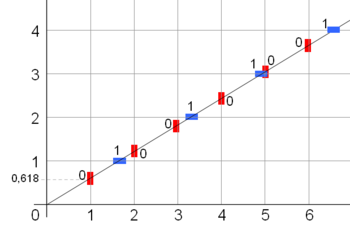
\includegraphics[width=0.8\columnwidth]{images/Fibonacci_word_cutting_sequence.png}
    \caption{Characteristic Sturmian word with slope $\frac{1}{\phi}$}
    \label{fig:fib_word}
\end{figure}
\end{minipage}
}

Sturmian words are \textbf{automatic-sequences} meaning that there are automata which calculate their $n$-th digit given the number $n$ in a special numeration system called the Ostrowski numeration system.

% \subsection*{Automata}
% \end{mdframed}
% 	\begin{definition}A \textbf{nondeterministic finite automaton}, or briefly an nfa, over alphabet $\Sigma$ is a quadruple $A = (S, I, T, F)$, where
% 	\begin{itemize}
% 		\setlength{\itemsep}{-30pt}
% 		\item $S$ is a finite nonempty set called the set of \textbf{states}.\\
% 		\item $I$ is a subset of $S$ called the set of \textbf{initial states}.\\
% 		\item $T \subset S \times \Sigma \times S$ is a nonempty set called the \textbf{transition table} or \textbf{transition diagram}.\\
% 		\item $F$ is a subset of $S$ called the set of \textbf{final states}.
% 	\end{itemize}
% \end{definition}

% \begin{definition}
% A \textbf{run} of A is a sequence $s_1...s_{n+1}$ on $u=\delta_1 ... \delta_n$ so that $s_1 \in I$ and $(s_i, \delta_i, s_{i+1}) \in T$.
% \end{definition}

% \begin{definition}
% % An input $u = \delta_1 ... \delta_n$ is \textbf{accepted} by $A$ if the last state of the run of $A$ on $u$ is in $F$.\\
% A string $u$ is \textbf{accepted} by $A$ if the last state of the run of $A$ on $u$ is in $F$.\\
% \end{definition}

\begin{mdframed}[style=MyFrame]
\subsection*{Numeration Systems}
\end{mdframed}
\begin{definition}A \textbf{numeration system} is a method used to represent numbers in which each digit represents a unique base value. Some examples of common systems are binary, decimal, and Ostrowski numerations.
\end{definition}
\begin{definition}
An \textbf{Ostrowski-$\alpha$ numeration} is a numeration system where the base values are calculated from the continued fraction of $\alpha$, denoted $[a_0; a_{1},a_{2}, \ldots]$.

The base values $q_{n}$ of an Ostrowski numeration are defined recursively by{
\setlength{\abovedisplayskip}{3pt}
\setlength{\belowdisplayskip}{3pt}
$$q_{n}=a_{n}q_{n-1}+q_{n-2} \text{ when } n \ge 2, \text{ where } q_{1}=a_1 \text{ and } q_{0}=1$$}

A string $b_n\dots b_3b_2b_1$ is a valid representation in an Ostrowski numeration system, if it satisfies:
\begin{itemize}
\item \textbf{constraint 1.} For all $n\ge 2$, $b_n\le a_n$, and $b_1 < a_1$
\item \textbf{constraint 2.} For all $n\ge 2$, if $b_{n} = a_{n}$, then $b_{n-1} = 0$.
\end{itemize}
\end{definition}

For example, when $\alpha = \sqrt[~]{2} = [1;2,2,2\dots]$, the base values are $1, 2, 5, 12, 29, 70, 169, \dots$.\\
$112020$ would be a valid representation in the Ostrowski-$\sqrt[~]{2}$ numeration system and would have value equal to $127$ in base-$10$.\\
$112100$ would not be a valid representation because it violates constraint 2 by having a 2 followed by a 1, $112030$ violates constraint 1 by having a 3 on the fourth digit. 
Similarly, $112030$ is not a valid representation in the Ostrowski-$\sqrt[~]{2}$ numeration system.\\

\begin{mdframed}[style=MyFrame]
\subsection*{Walnut Software}
\end{mdframed}

%Explanation of how Walnut works
Walnut is a theorem-prover developed by Hamoon Mousavi in 2016. 
It takes any \emph{first-order logic with addition and comparison} then outputs an automaton associated with it. 

In addition, Walnut can use any numeration system, as long as the following three automata are provided:
\begin{itemize}
\item A \emph{recognition automaton} that only accepts valid numbers in that numeration system.
\item An \emph{addition automaton} that only accepts triples $(a,b,c)$ such that $a+b=c$.
\item A \emph{comparison automaton} that only accepts pairs $(a,b)$ such that $a<b$.
\end{itemize}

The comparison automaton is auto-generated, and one can check that the automaton in \emph{Figure 1} accepts input that meets constraints 1 and 2. 
We produce the addition automaton as described in the next section.

\columnbreak

% \centerline{
% \begin{minipage}{.4\columnwidth}
% %Insert Picture of automaton
% \begin{figure}
% 	\centering
%     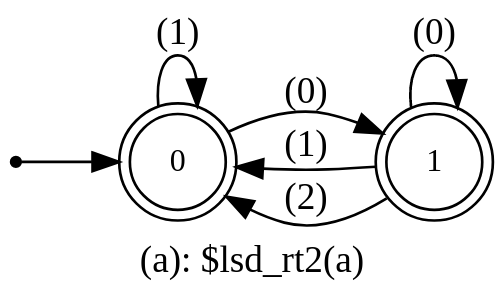
\includegraphics[width=\columnwidth]{images/lsd_rt2.png}
%     \caption{Ostrowski-$\sqrt[~]{2}$ Recognition}
%     \label{fig:lsd_rt2}
% \end{figure}
% \end{minipage}
% }

%%%%%%%%%%%%%%%%%%%%%%%%%%%%%%%%%%%%%
%% New Section
%%%%%%%%%%%%%%%%%%%%%%%%%%%%%%%%%%%%%
\section*{Bounded Sturmian Words and Corresponding Automata}

For some positive integer $k$, call $\alpha_{<k}$ the set of \textit{$k$-bounded continued fractions}, whose members are the irrational number for which each coefficient of its continued fraction representation is less than $k$.

A \textit{$k$-bounded Ostrowski numeration system} is an Ostrowski numeration system for some $\alpha \in \alpha_{<k}$. 
A \textit{$k$-bounded Sturmian Word} is a Sturmian word whose slope is in $\alpha_{<k}$.
Given $k$, we can then define a single addition automata for every $k$-bounded Ostrowski numeration system at once, by defining four sub-algorithms, which combine to form the bounded addition automaton.
The basic algorithms were originally defined in Hieronymi and Terry's paper ``Ostrowski Numeration Systems,'' and we have since modified the algorithms to work for any $k$-bounded Ostrowski numeration system.

\begin{itemize}
\item Algorithm 0 adds the operands.
\item Algorithm 1 checks constraint 1.
\item Algorithms 2 and 3 check constraint 2.
\end{itemize}

With the following predicate, we can create the addition automaton, shown in Figure~\ref{fig:rt2_addition}: {
$$\exists y,x,w ~\text{alg}_0(a,b,w) ~\& ~\text{alg}_1(\alpha,w,x) ~\& ~\text{alg}_2(\alpha,x,y) ~\& ~\text{alg}_3(\alpha,y,c)$$}

\begin{minipage}{.45\columnwidth}
%Insert Picture of automaton

\begin{figure}
	\centering
    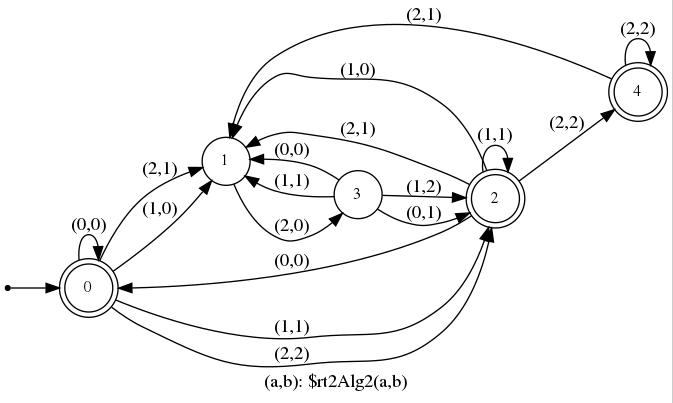
\includegraphics[width=\columnwidth]{rt2Alg2_gv.jpg}
    \caption{Algorithm 2 of Ostrowski-$\sqrt[~]{2}$ (least significant digit first)}
    \label{fig:rt2_alg2}
\end{figure}
\end{minipage} ~~ %
\begin{minipage}{.45\columnwidth}
\begin{figure}
	\centering
    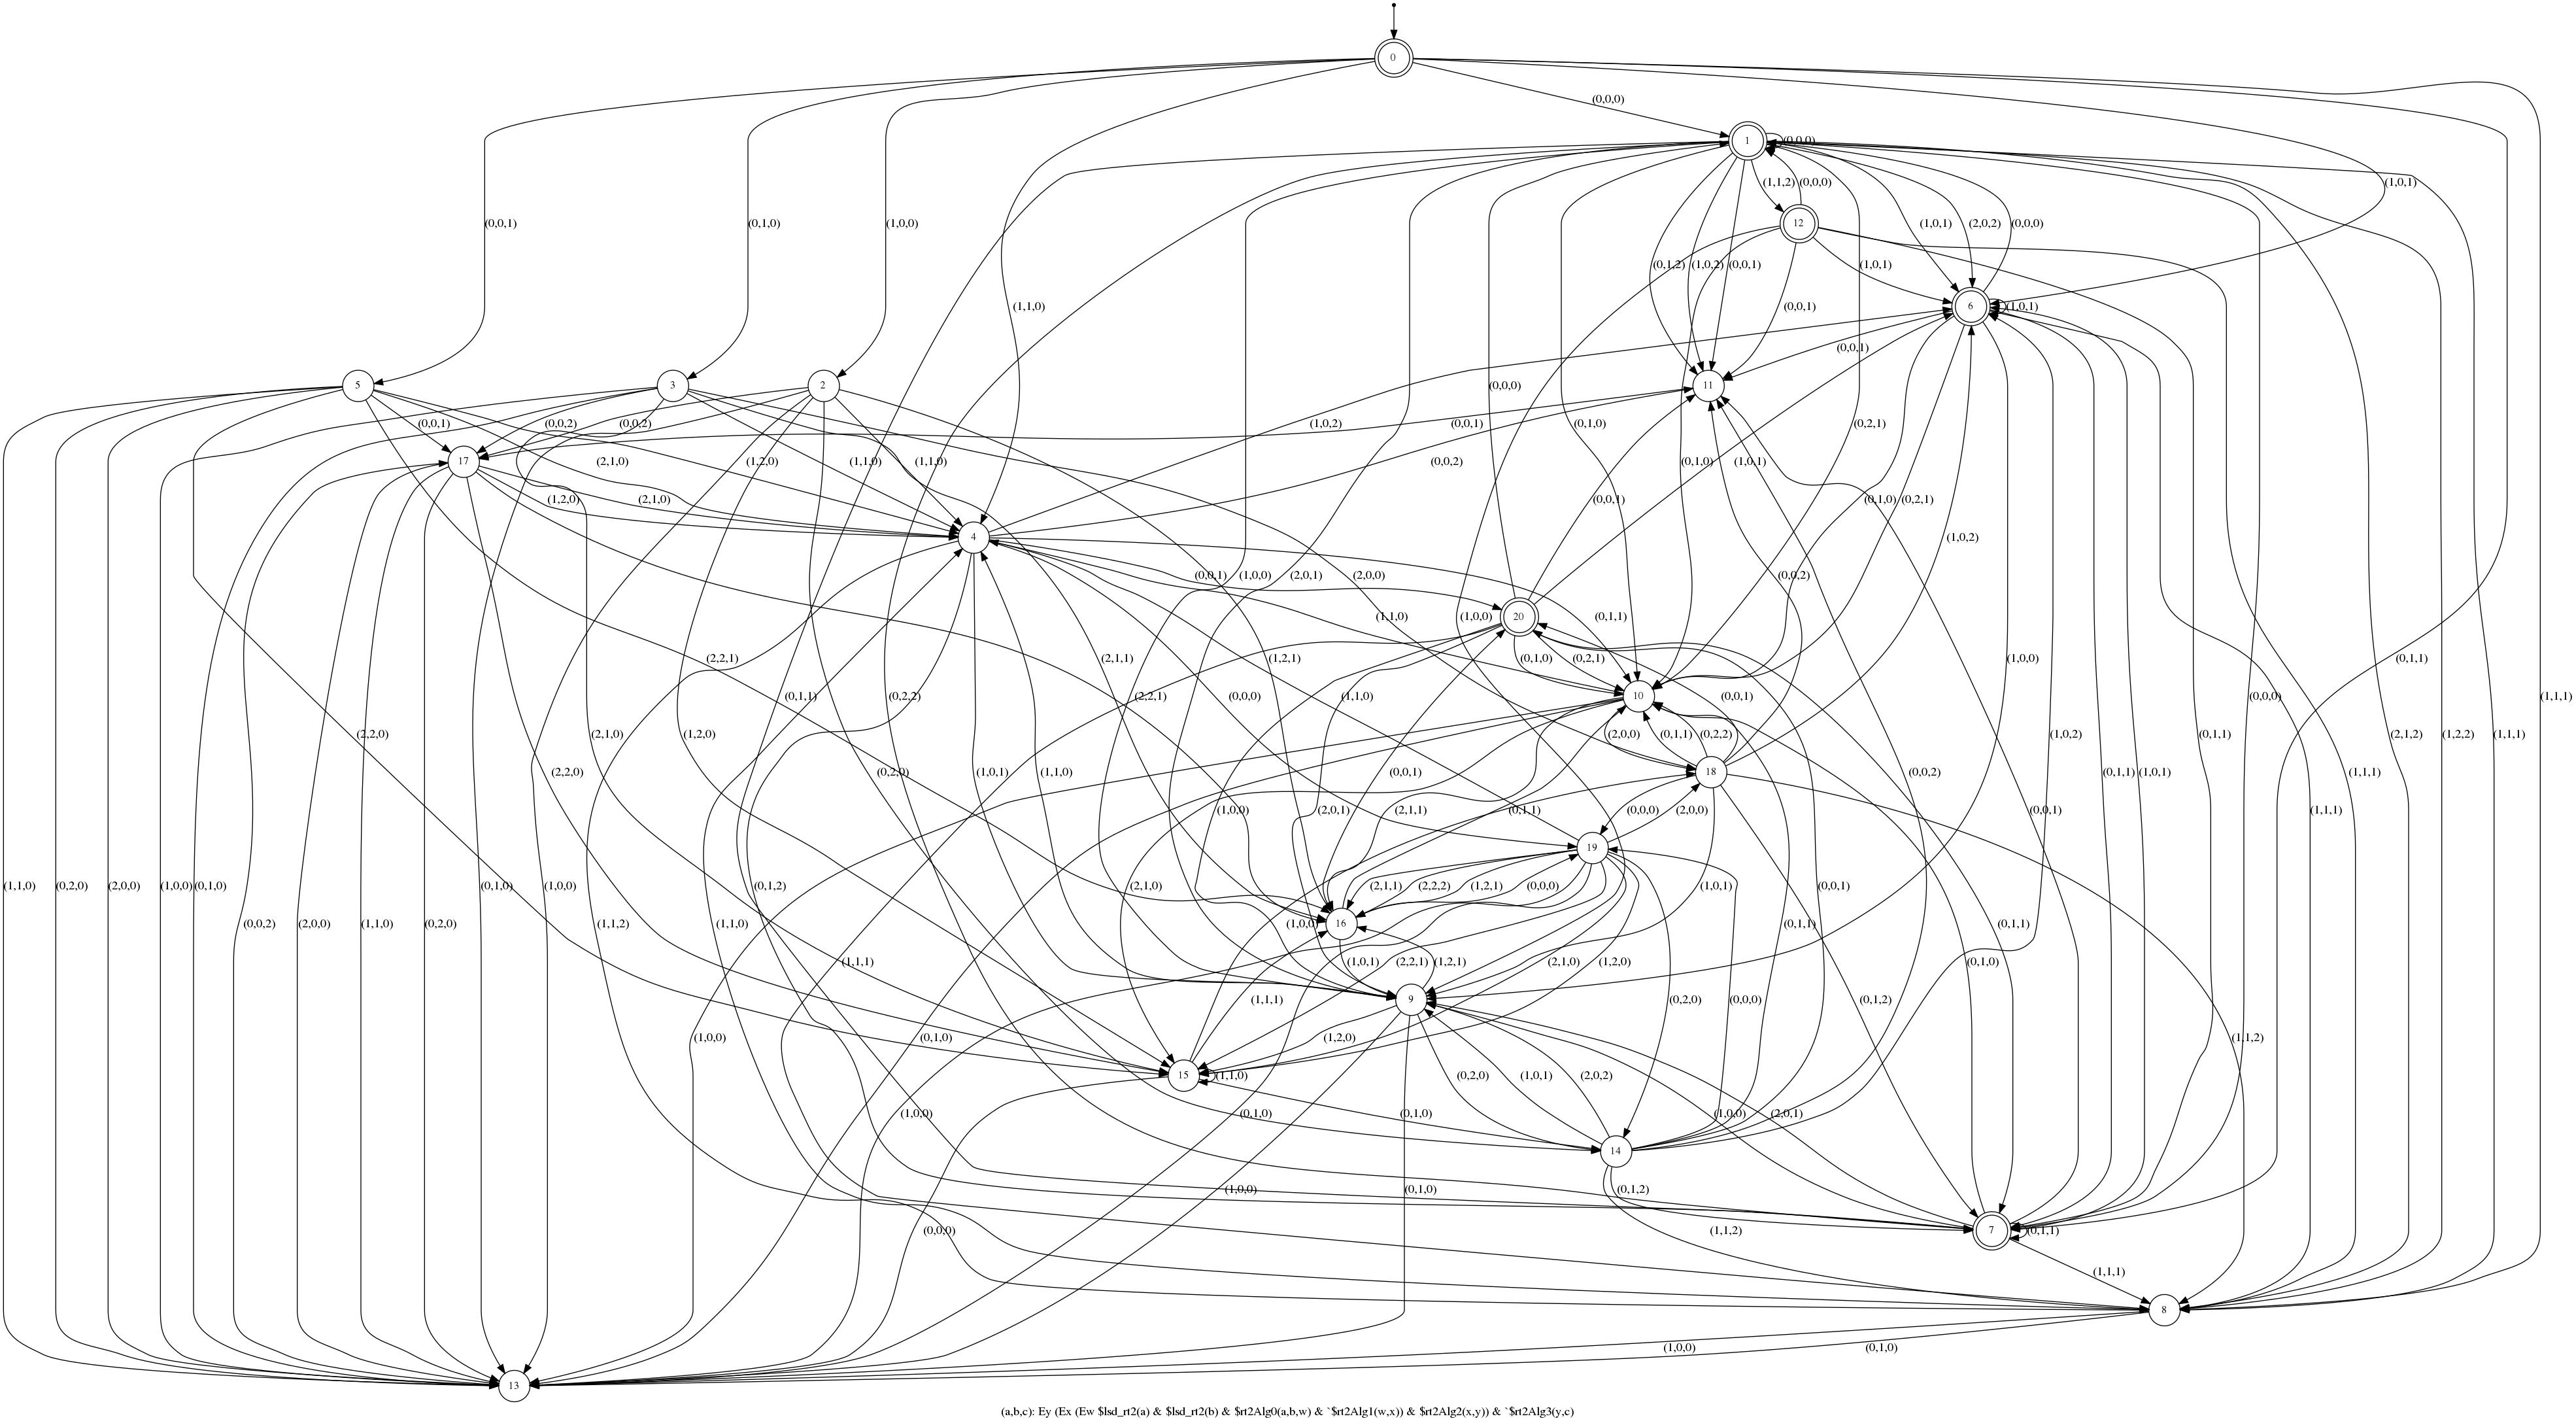
\includegraphics[width=\columnwidth]{lsd_rt2_addition_gv.jpg}
    \caption{Ostrowski-$\sqrt[~]{2}$ Addition}
    \label{fig:rt2_addition}
\end{figure}
\end{minipage}

The bounded addition automata are much too large to show: for $k=2$, the resulting automaton has 23 states and 245 transitions, and for $k=3$, it has 23 states and 605 transitions.
We are able to produce automata for up to $k=7$, which has nearly 5000 transitions.
However, Figures~\ref{fig:rt2_alg2} and~\ref{fig:rt2_addition} show similar automata for the case of $\alpha = \sqrt{2}$.

% The automaton for $k=2$ is shown in Figure~\ref{fig:add_2_automaton}.

% \centerline{
% \begin{minipage}{.4\columnwidth}
% %Insert Picture of automaton
% \begin{figure}
% 	\centering
%     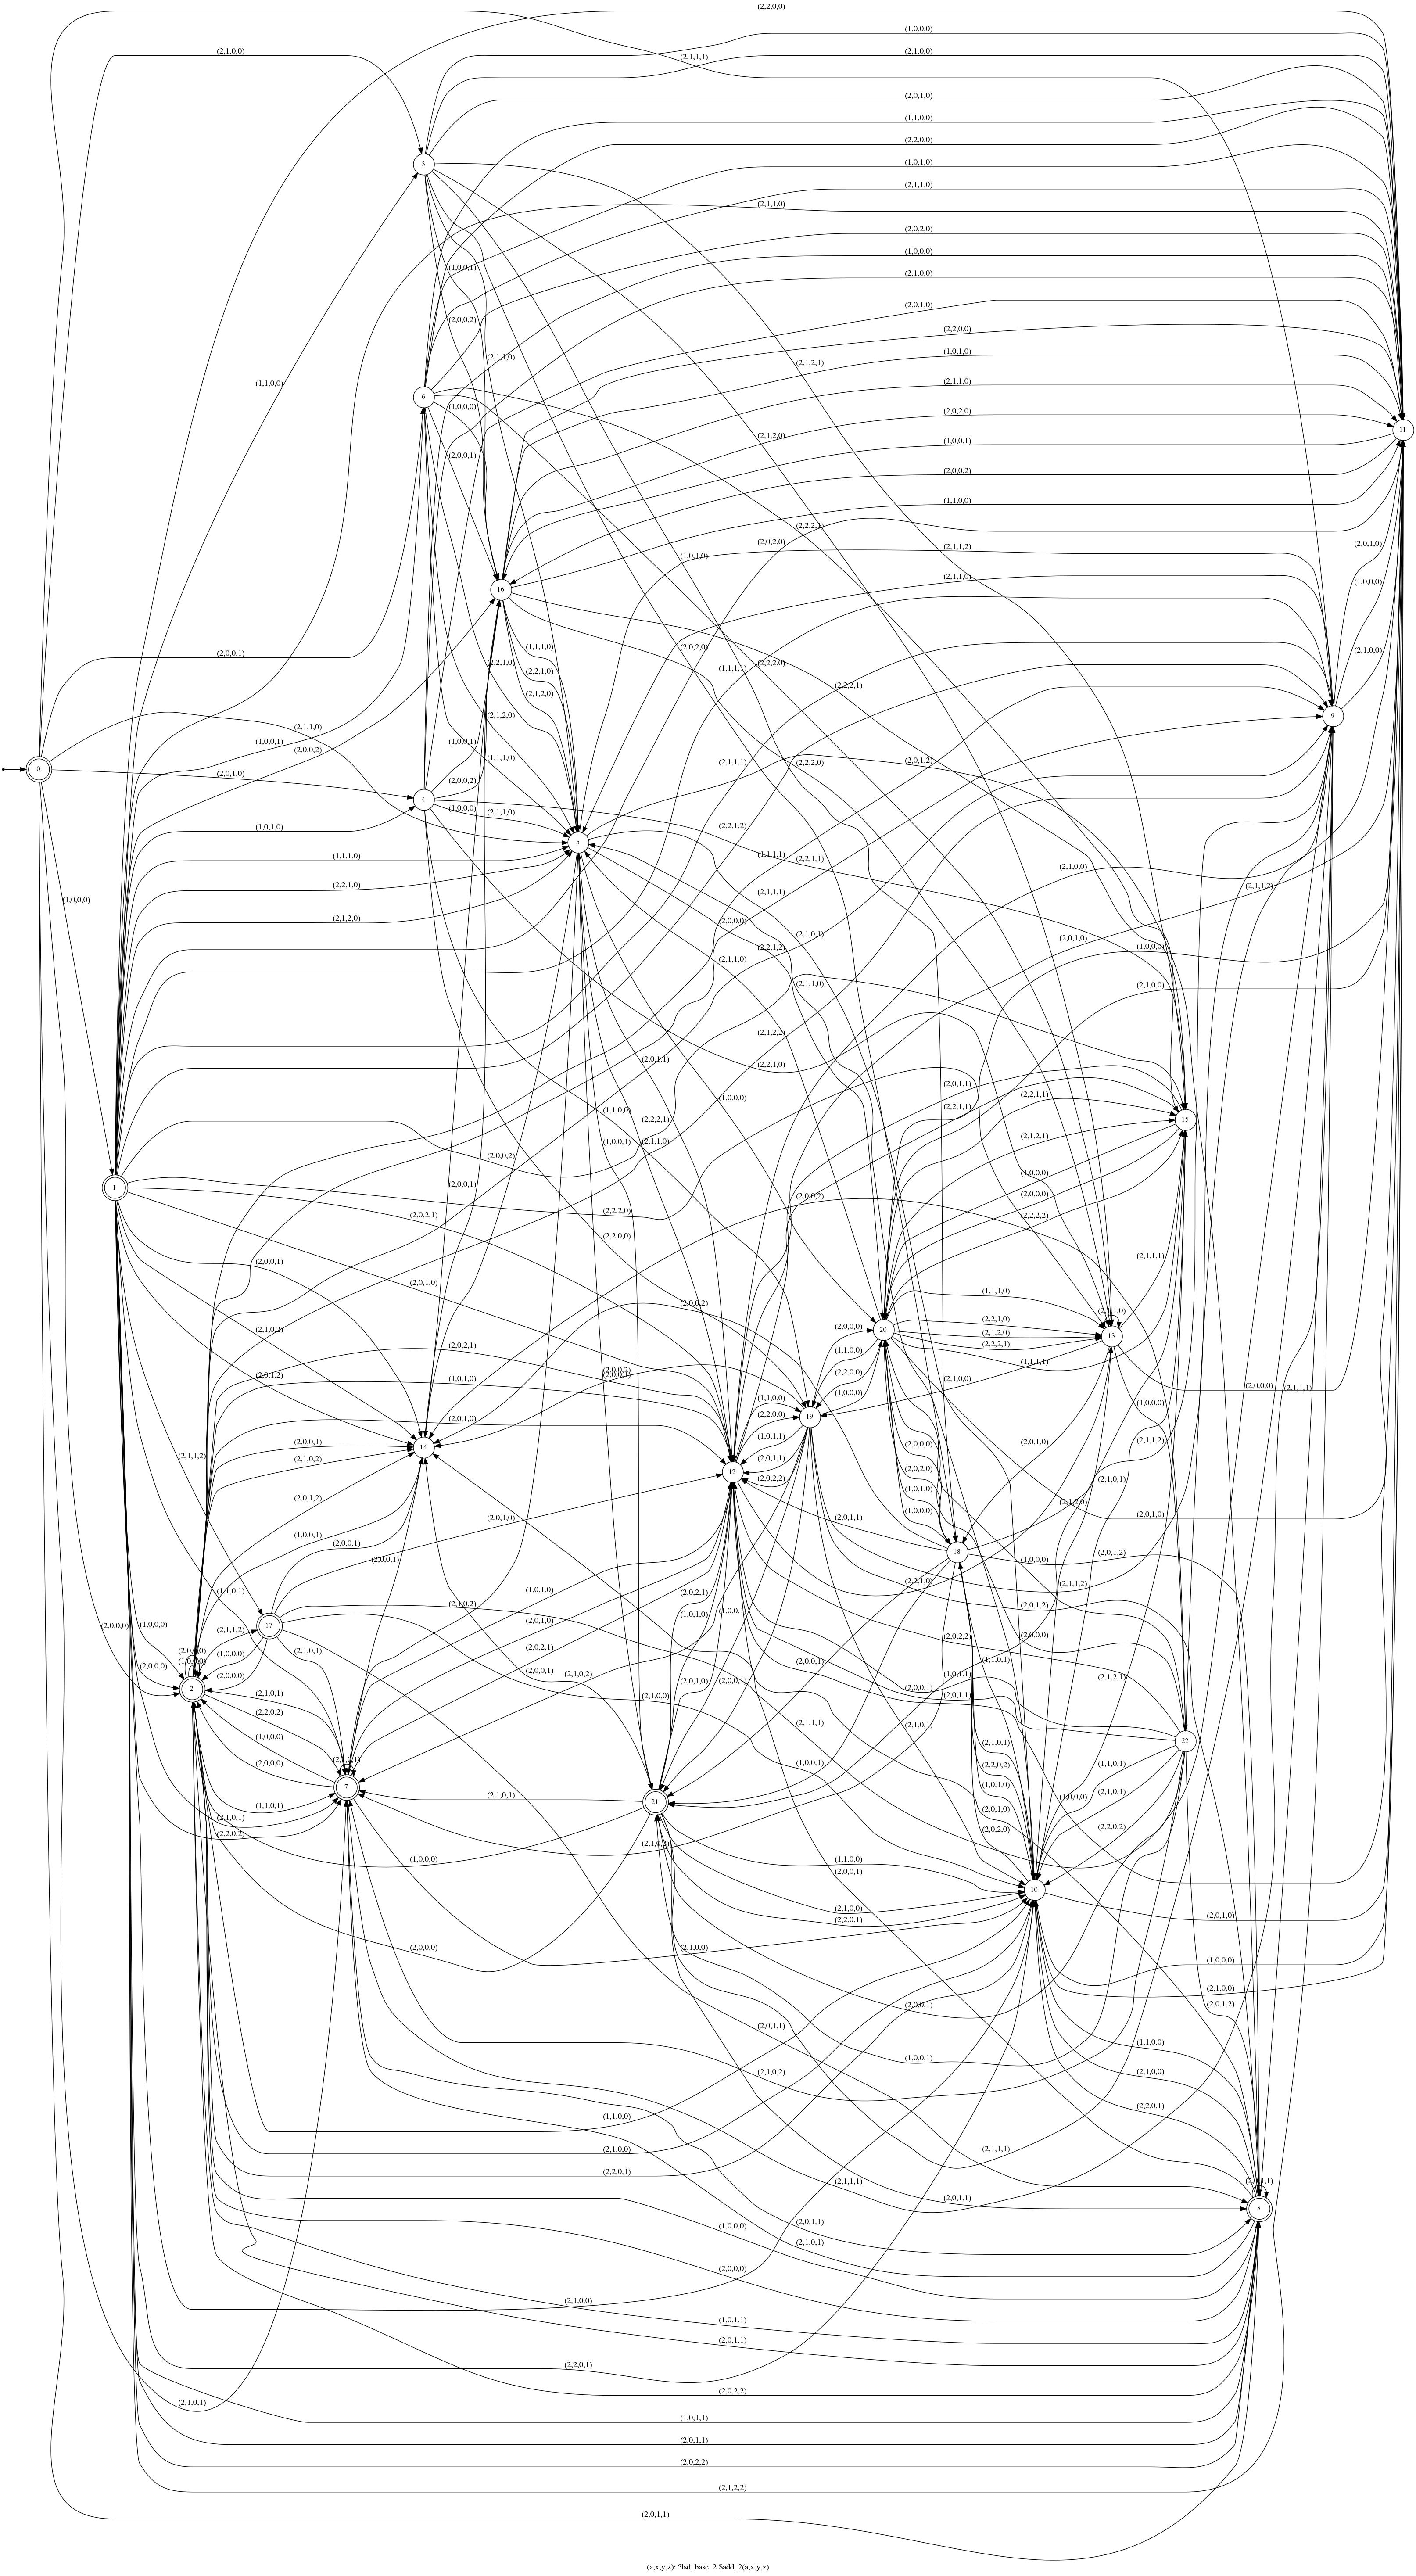
\includegraphics[width=\columnwidth]{add_2.jpg}
%     \caption{$2$-bounded Ostrowski addition automaton}
%     \label{fig:add_2_automaton}
% \end{figure}
% \end{minipage}
% }

\begin{mdframed}[style=MyFrame]
\subsection*{Automata Verification}
\end{mdframed}

In addition to generating the automata, we also use Walnut to prove that our definition correctly defines addition according to the standard recursive definition of addition:

$$0 + n = n; \quad \quad a + (b + 1) = (a + b) + 1\\$$

We can define the successor without reference to addition as follows:

\begin{definition}
Let $\alpha \in \alpha_{<k}$ and let $x$ be the valid Ostrowski-$\alpha$ representation of some natural number.
Then the \textbf{successor} of $x$ is a string $y$ such that $x <_{\alpha} y$ and for all $k$, either $k \leq_{\alpha} x$ or $y \leq_{\alpha} k$.
\end{definition}

Then by checking the base case and the inductive case, we can use Walnut to prove that our automata are correct.

% \begin{mdframed}[style=MyFrame]
% \subsection*{Automaton for Algorithm 1}
% \end{mdframed}
%     \begin{definition}
%     $\text{alg}_1(\alpha = [a_0; a_1,a_2,\dots])$ is a nondeterministic finite automaton $\{S,I,T,F\}$ over $\Sigma$ where:
%     \begin{itemize}
%     \item \textbf{alphabet} $\Sigma = \left\{(s,t) : 0\le s \le 2 ~max(a_i),0\le t \le max(a_i) \right\}$.
%   \item set of \textbf{states} $S = \left\{\left(\begin{bmatrix}a&b&c\\d&e&f\end{bmatrix},g,i\right)\right\}$. The matrix represents the input, $g$ is a carry number that is 0 or 1, and $i$ represents the position of $c$ and $f$ in the continued fraction.
%   \item set of \textbf{initial states} I = $\left\{\left(\begin{bmatrix}0&0&0\\0&0&0\end{bmatrix},0,i\right)\right\}$ for all integers $i> 0$.
%   \item set of \textbf{final states} F = $\left\{\left(\begin{bmatrix}a&b&c\\d&e&f\end{bmatrix},0,0\right):B(a,b,c)=(d,e,f)\right\}$ where $B$ does not change the represented values between $(a,b,c)$ and $(d,e,f)$ while the latter satisfies constraint 1.
%   \item \textbf{transition table} :  $\left(\left(\begin{bmatrix}a&b&c\\d&e&f\end{bmatrix},g,i\right), \begin{pmatrix}s\\t\end{pmatrix}, \left(\begin{bmatrix}b'&c'&s'\\e&f&t\end{bmatrix},g',i-1\right)  \right) \in T$ if $(a+g,b,c,s,g)$ and $(d,b',c',s')$ represent the same value, and the latter satisfies constraint 1.
%   \end{itemize}
% \end{definition}
% \begin{mdframed}[style=MyFrame]
% \subsection*{Automaton for Algorithm 2}
% \end{mdframed}
% \begin{definition}
%     $\text{alg}_2(\alpha = [a_1,a_2,\dots])$ is a nondeterministic finite automaton $\{S,I,T,F\}$ over $\Sigma$ where:
%     \begin{itemize}
%     \item \textbf{alphabet} $\Sigma = \left\{(s,t) : 0\le s,t \le max(a_i) \right\}$
%    \item \textbf{set of states} $S = \left\{\left(\begin{bmatrix}a&b\\c&d\end{bmatrix},i\right)\right\}$. The matrix represents the input,  and $i$ represents the position of $b$ and $d$ in the continued fraction.
%    \item \textbf{initial state} I = $\left\{\left(\begin{bmatrix}0&0\\0&0\end{bmatrix},-2\right)\right\}$.
%    \item \textbf{set of final states} F = $\left\{\left(\begin{bmatrix}a&b\\c&d\end{bmatrix},i\right):a=c,b=d, i\ge0\right\}$.
%    \item \textbf{transition table} :  $\left(\left(\begin{bmatrix}a&b\\c&d\end{bmatrix},i\right), \begin{pmatrix}s\\t\end{pmatrix}, \left(\begin{bmatrix}s'&a'\\t&c\end{bmatrix},i+1\right)  \right) \in T$ if the represented value of $(s,a,b)$ and $(s',a',d)$ are the same, and the latter satisfies constraint 2.
%    \end{itemize}
% \end{definition}

%Here we used \section instead of \section*, so it has a number

%%%%%%%%%%%%%%%%%%%%%%%%%%%%%%%%%%%%%
%% New Section
%%%%%%%%%%%%%%%%%%%%%%%%%%%%%%%%%%%%%
\begin{mdframed}[style=MyFrame]
\subsection*{Example of addition algorithm in Ostrowski-$\sqrt[~]{2}$}
\end{mdframed}
\begin{minipage}{\columnwidth}
%Insert explanation of Algorithms 1,2 and 3, etc.

Suppose we want to add $103_{10}$ and $132_{10}$ in Ostrowski numeration with $\alpha = \sqrt[~]{2}= [1; 2,2,2,\dots].$
\begin{enumerate}
\item Convert into Ostrowski representation:\\
$109_{10} = 0\times1_{10}+0\times2_{10}+2\times5_{10}+0\times12_{10}+1\times29_{10}+1\times70_{10}= 0110200_{\sqrt[]{2}}$
\\
$138_{10} = 0\times1_{10}+0\times2_{10}+2\times5_{10}+0\times12_{10}+2\times29_{10}+1\times70_{10} = 0120200_{\sqrt[]{2}}$
\item Run Algorithm 0 (add operands): $0110200 + 0120200 \Rightarrow 0230400$.
\item Run Algorithm 1 (check constraint 1): $0230400 \Rightarrow 1020400 \Rightarrow 1021111$.
\item Run Algorithms 2 and 3 (check constraint 2): $1021111 \Rightarrow 1100111$. (Try this on \emph{Figure 2}.)
\end{enumerate}
Therefore, $0110200_{\sqrt[]{2}}+0120200_{\sqrt[]{2}}=1100111_{\sqrt[]{2}}$.\\

% Verify:
% $1100111_{\sqrt[]{2}}  = 1\times1_{10}+1\times2_{10}+1\times5_{10}+1\times70_{10}+1\times169_{10}$ = $247_{10} = 109_{10}+138_{10}$.\\

\end{minipage}

\columnbreak

%%%%%%%%%%%%%%%%%%%%%%%%%%%%%%%%%%%%%
%% New Section
%%%%%%%%%%%%%%%%%%%%%%%%%%%%%%%%%%%%%
\section*{Propositions Evaluated in Walnut}

By defining automata for $k$-bounded Ostrowski numeration systems, we are able to automatically decide propositions about infinite classes of Sturmian words all at once; previous work has only been able to automatically prove propositions about a single Sturmian word given its slope.
We then construct similar proofs to those in Du, Mousavi, Schaeffer, and Shallit's paper ``Decision Algorithms for Fibonacci-Automatic Words, with Applications to Pattern Avoidance'', but now our proofs are much more general.

% \vspace*{0.4em}
% \begin{definition}
% The \textbf{characteristic Sturmian word with slope $\sqrt[~]{2}$}, which we denote as $C_2$, is the infinite word obtained as the limit of the sequence of \textbf{standard words} $s_n$ defined by{
% \setlength{\abovedisplayskip}{3pt}
% \setlength{\belowdisplayskip}{3pt}
% $$ s_n=s^{d_n}_{n-1}s_{n-2} \text{ when } n\ge 2, \text{ where } s_1= 0^{d_1-1}1 \text{ and } s_0=0.$$}
% \end{definition}

% By having built the Ostrowski-$\sqrt[~]{2}$ numeration system and the automatic word $C_2$ in Walnut, we may use the command $C2[i]$ to return the $i^{th}$ digit of $C_2$.\\

\begin{mdframed}[style=MyFrame]
\subsection*{Example Theorem}
\end{mdframed}

A factor $z$ is called a \textbf{square} if can be written as $z = xx$ for some word $x$.
The \textbf{order} of a square is the length of the repeated part, $|x|$.

\textbf{Theorem:} \emph{For all $2$-bounded Sturmian words, the orders of squares are of the form $(11+2+1)0^*$ in their respective numeration system (e.g., $1,2,11,10,20,110,\ldots$).}

\textbf{Proof:} We encode the property that there is a square of order $n > 0$ in $C_{\alpha}$ as follows, where $C_{\alpha}(i,n)$ denotes the factor of length $n$ starting at index $i$: $\exists i > 0, C_{\alpha}(i,n) = C_{\alpha}(i+t,n)$.

\centerline{
\begin{minipage}{.4\columnwidth}
\begin{figure}
	\centering
    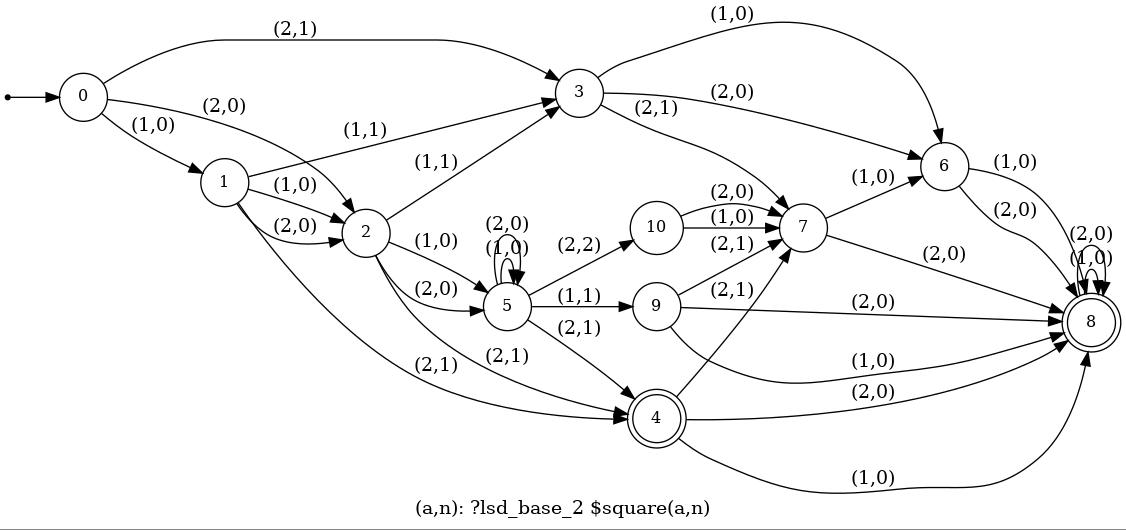
\includegraphics[width=\columnwidth]{square.jpg}
    \caption{Orders of squares in $2$-bounded Sturmian words}
    \label{fig:square_2}
\end{figure}
\end{minipage}
}

The resulting automata is shown above in Figure~\ref{fig:square_2}.
Using Walnut we can create an automata that matches the regular expression $E_k = (11+2+1)0^*$ to check the following predicate:

\begin{equation*}\label{def:square-conj}
\forall \alpha \in \alpha_{<k} \forall n, \text{if $n$ is the order of a square in $C_{\alpha}$, then $n \in L(E_k)$}.
\end{equation*}

A similar pattern holds for $k$-bounded Sturmian words for higher $k$ (prove for up to $k=5$):

\textbf{Conjecture:} The orders of the squares in $k$-bounded Sturmian words are of the form $E_k = (1+2+\cdots+(k-1))(1+\epsilon)0^*$.

\begin{mdframed}[style=MyFrame]
\subsection*{More Theorems}
\end{mdframed}

We are able to prove theorems about many other properties of $k$-bounded Sturmian words using our automata and Walnut, including:

\begin{itemize}
    \item They are aperiodic for $k=1,2,3,4,5$.
    \item They contain a finite number of $0$ and $1$-approximate antisquares for $k = 2$.
    \item They do not contain $(k+3)$-th powers for $k=2$.
    \item They contain unbordered factors of lengths $(1+2+\cdots+k)0^*$ for $k=2,3,4,5$.
    \item They contain grouped factors for $k=2,3$.
\end{itemize}

% \textbf{Theorem}: \textbf{$C_2$} \textit{contains fourth powers.}
% \\

% \textbf{Proof}: We create the following predicate that accepts the length $n$ of fourth powers in $C_2$
% \setlength{\abovedisplayskip}{3pt}
% \setlength{\belowdisplayskip}{3pt}
% $$(n > 0) \land \exists i \; \forall t<3n \;C_2[i+t] = C_2[i+n+t]$$
% We then translate the predicate into one that Walnut recognizes:
% % \setlength{\abovedisplayskip}{3pt}
% % \setlength{\belowdisplayskip}{3pt}
% $$ ? \text{msd}\_\text{rt2} ((n>0)~\&~(Ei~At (t<3 \ast n => C2[i+t] = C2[i+n+t])))$$
% For this predicate, Walnut generates the following automaton:
% \\
% \begin{figure}
% \centering
% 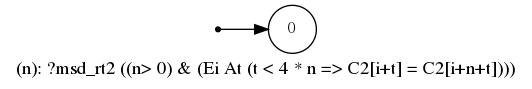
\includegraphics[width=0.7\columnwidth]{theorem5_1_gv.jpg}
%     \caption{Automaton for the Theorem}
%     \label{fig:Theorem}
% \end{figure}
% which means that there are fourth powers of length $100_{\sqrt[~]{2}},1000_{\sqrt[~]{2}},10000_{\sqrt[~]{2}},\dots$.
%Maybe a future work section here?
\section*{Future Work}
\begin{itemize}
\item Continue to prove theorems regarding characteristic Sturmian words.
% \item Investigate the critical exponent of infinite balanced words. % Maybe remove this?
\item Find a more space-efficient algorithm to generate automata for bounded Ostrowski addition.
\item Provide a general automaton for Ostrowski numeration accepting any irrational $\alpha$.
\end{itemize}

\vspace*{-10pt}  %change to -10
\section*{References}

{\footnotesize [1] Khoussainov, Bakhadyr.Nerode, Anil. (2001) \emph{Automata Theory and its Applications}, MA : Birkh\"auser Boston
}

{\footnotesize [2] Rampersad, Narad. Shallit, Jeffrey and  Vandomme, Elise. (2018) \emph{Critical exponents of infinite balanced words}, Canada
}

{\footnotesize [3] Du, Chen Fei. Mousavi, Hammoon. Schaeffer, Luke and Shallit, Jeffrey. (2014) \emph{Decision Algorithms for Fibonacci-Automatic Words, with Applications to Pattern Avoidance}
}

{\footnotesize [4] Hieronymi, P., \& Terry Jr, A. (2018). \emph{Ostrowski Numeration Systems, Addition, and Finite Automata}. Notre Dame Journal of Formal Logic, 59(2), 215-232.
}

\vspace*{2cm} %This will change to -5
\centerline{\emph{
%Support for this project was provided by the Illinois Geometry Lab and the Department of Mathematics at the University of Illinois at Urbana-Champaign.
}}
\end{multicols}

\end{document}
